% -------------------
% --- Definicia zakladnych pojmov
% --- Vyplnte podla vasho zadania
% -------------------
\def\mfrok{2016}
\def\mfnazov{Design and implementation of an RFID access control system}
\def\mftyp{Bachelor's Thesis}
\def\mfautor{Kamila Součková}
\def\mfskolitel{RNDr.~Richard Ostertág, PhD.}

%ak mate konzultanta, odkomentujte aj jeho meno na titulnom liste
%\def\mfkonzultant{tit. Meno Priezvisko, tit. }

\def\mfmiesto{Bratislava, \mfrok}

%aj cislo odboru je povinne a je podla studijneho odboru autora prace
\def\mfodbor{2508 Informatics}
\def\program{ Informatics }
\def\mfpracovisko{ Department of Computer Science }

% -------------------
% --- Obalka ------
% -------------------
\thispagestyle{empty}

\begin{center}
\sc\large
Comenius University in Bratislava\\
Faculty of Mathematics, Physics and Informatics

\vfill

{\LARGE\mfnazov}\\
\mftyp
\end{center}

\vfill

{\sc\large
\noindent \mfrok\\
\mfautor
}

\eject % EOP i
% --- koniec obalky ----

% -------------------
% --- Titulný list
% -------------------

\thispagestyle{empty}
\noindent

\begin{center}
\sc
\large
Comenius University in Bratislava\\
Faculty of Mathematics, Physics and Informatics

\vfill

{\LARGE\mfnazov}\\
\mftyp
\end{center}

\vfill

\noindent
\begin{tabular}{ll}
Študijný program: & \program \\
Študijný odbor: & \mfodbor \\
Školiace pracovisko: & \mfpracovisko \\
Školiteľ: & \mfskolitel \\
% Konzultant: & \mfkonzultant \\
\end{tabular}

\vfill


\noindent \mfmiesto\\
\mfautor

\eject % EOP i


% --- Koniec titulnej strany


% -------------------
% --- Zadanie z AIS
% -------------------
% v tlačenej verzii s podpismi zainteresovaných osôb.
% v elektronickej verzii sa zverejňuje zadanie bez podpisov

\newpage
\thispagestyle{empty}
\hspace{-2cm}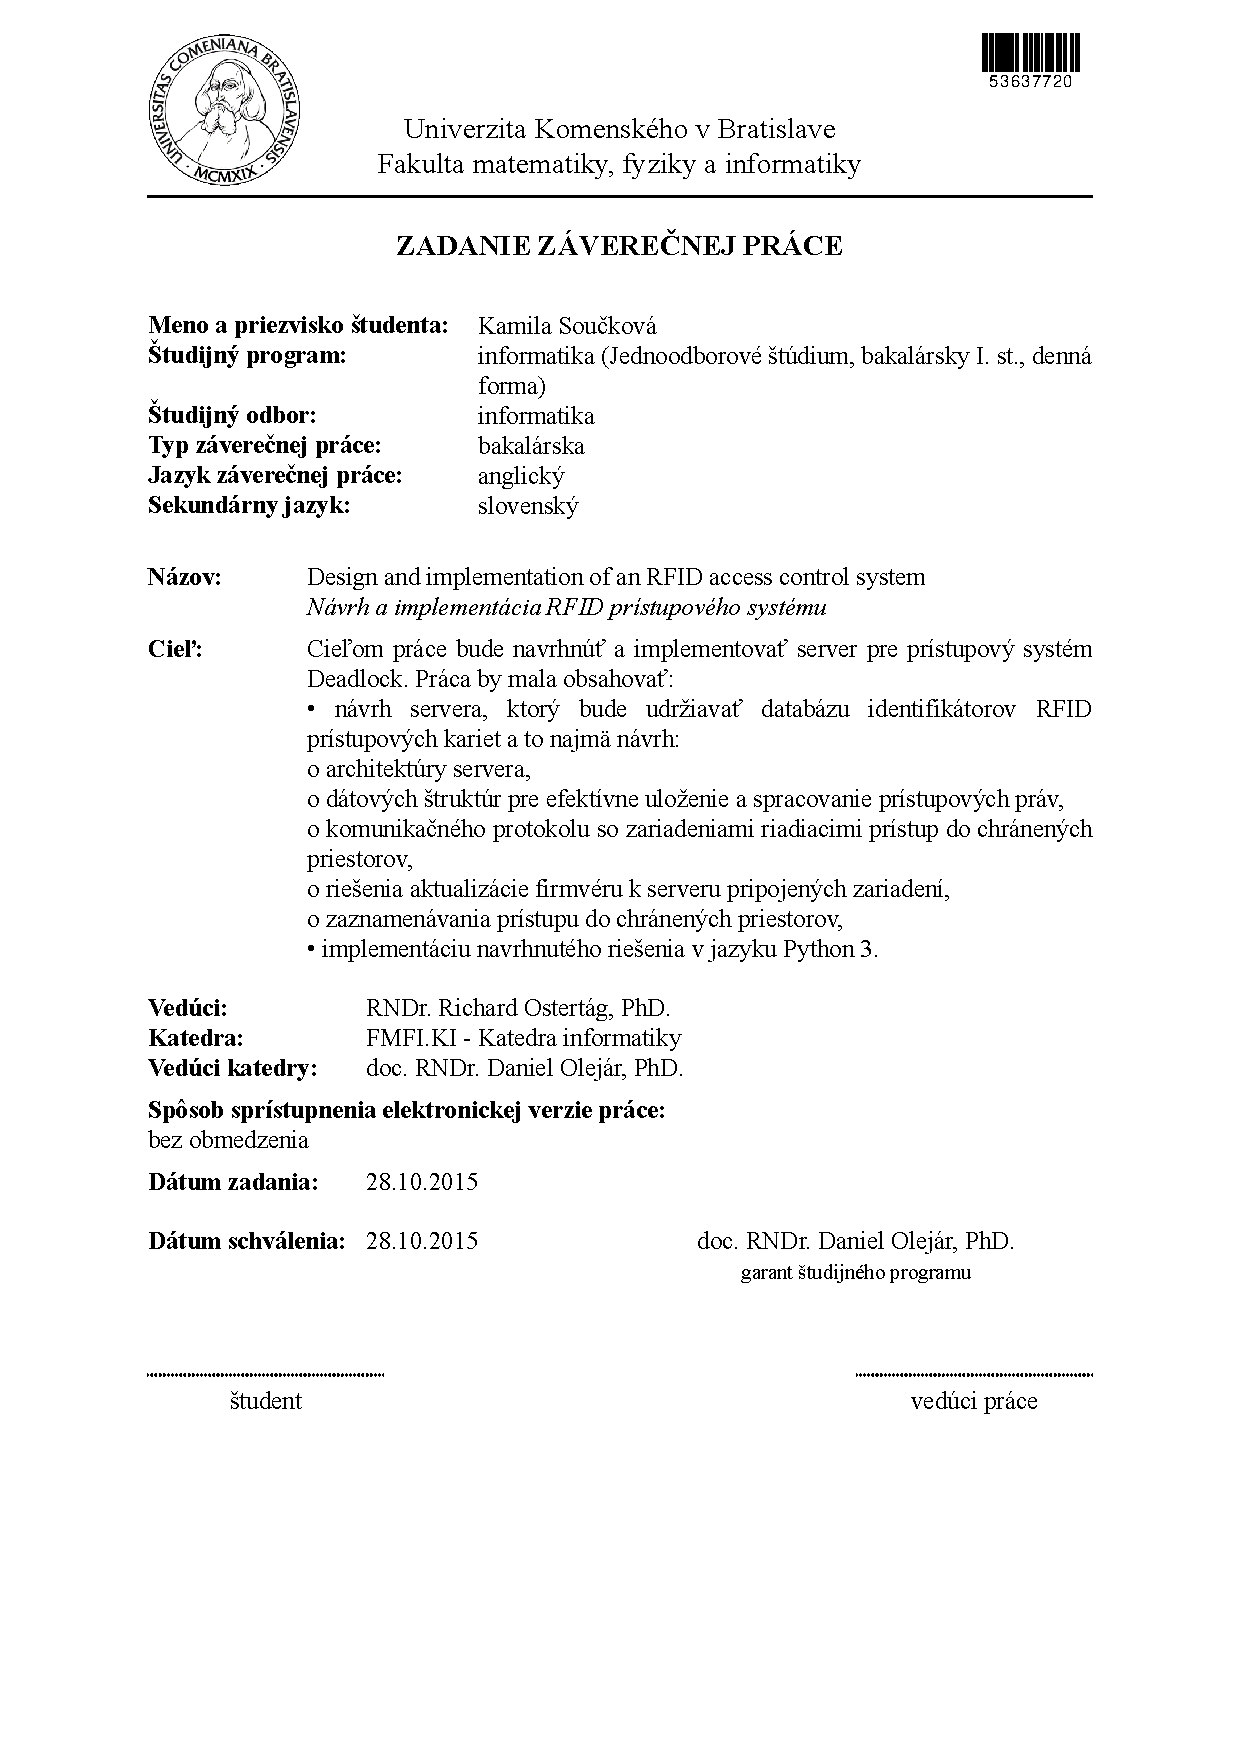
\includegraphics[width=1.1\textwidth]{src/img/zadanie}

% --- Koniec zadania

\frontmatter

% -------------------
%   Poďakovanie - nepovinné
% -------------------
\setcounter{page}{3}
\newpage
~

\vfill
\noindent\textbf{Acknowledgements:} I would like to thank RNDr.~Jaroslav Janáček, PhD., RNDr.~Richard Ostertág, PhD., and Mgr.~Tomáš Vinař, PhD.~for their valuable input on the design and requirements of the system. Without their insightful discussions, Deadlock would lack the strengths that make it unique, such as reliability and simplicity.

I would also like to thank Adam Dej, who designed and is at the time of writing implementing the embedded devices. Deadlock would not exist without him.

Finally, I would like to thank Michal Hanula and RNDr.~Richard Královič, PhD.~for listening and asking questions. They helped me to see things from a different viewpoint, which led to considerable improvements.

% --- Koniec poďakovania

% -------------------
% --- Abstrakt - Anglicky
% -------------------
\newpage
\section*{Abstract}

Project Deadlock is a system that controls access to a number of points of
access (e.g.~doors, appliances) using RFID cards. Deadlock is designed for
security and reliability, assuming untrusted and unreliable network. It is fully open-source and open-hardware, and designed  to be flexible, maintainable, and cost-effective. It is easy to integrate with existing systems and customize to the needs of the user.

This thesis first lists the requirements and introduces the high-level design choices we made in order to fulfill them.
It then focuses on the design and implementation choices of some parts of the system.
We start with the design and implementation of the system's communication protocol, focusing on the conflicting requirements of reliability, extensibility and simplicity.
Next, we describe the access rules format and evaluation, especially the compromise of generality vs.~user-friendliness.
Third, we provide an overview of the server design and implementation.
We conclude with the future plans for Project Deadlock.

\paragraph*{Keywords:} access control, networked system design, network protocol design, reliable system design

% --- Koniec Abstrakt - Anglicky

% -------------------
%   Abstrakt - Slovensky
% -------------------
\newpage
\section*{Abstrakt}

Projekt Deadlock je systém na kontrolu prístupu do miestností alebo k zariadeniam na základe identifikáce RFID kartou.

Deadlock je navrhnutý s dôrazom na bezpečnosť a spoľahlivosť aj za použitia nezabezpečenej
a nespoľahlivej siete. Je plne open-source a open-hardware a navrhnutý s cieľom pružnosti,
udržiavateľnosti a cenovej efektivity. Je možné ľahko ho integrovať s existujúcimi systémami
a prispôsobovať požiadavkám používateľa.

Táto bakalárska práca vychádza z požiadaviek na systém a vysvetľuje základné
rozhodnutia pri jeho návrhu. Ďalej sa zameriava na rozhodnutia pri návrhu a implementácii
niektorých častí systému. Začíname návrhom a implementáciou použitého komunikačného protokolu,
dbajúc na to, aby súčasne vyhovoval
požiadavkám spoľahlivosti, rozšíriteľnosti a jednoduchosti. Ďalej popisujeme štruktúru
a spôsob vyhodnocovania prístupových pravidiel, pristavujúc sa najmä pri kompromise medzi všeobecnosťou,
jednoduchosťou a prívetivosťou pre používateľa. Pokračujeme prehľadom návrhu a implementácie servera.
Na záver popisujeme ďalšie plány projektu Deadlock.

\paragraph*{Kľúčové slová:} kontrola prístupu, návrh distribuovaného systému, návrh sieťového protokolu, návrh spoľahlivého systému
% --- Koniec Abstrakt - Slovensky


% -------------------
% --- Predhovor - v informatike sa zvacsa nepouziva
% -------------------
%\newpage
%\thispagestyle{empty}
%
%\huge{Predhovor}
%\normalsize
%\newline
%Predhovor je všeobecná informácia o práci, obsahuje hlavnú charakteristiku práce
%a okolnosti jej vzniku. Autor zdôvodní výber témy, stručne informuje o cieľoch
%a význame práce, spomenie domáci a zahraničný kontext, komu je práca určená,
%použité metódy, stav poznania; autor stručne charakterizuje svoj prístup a svoje
%hľadisko.
%
% --- Koniec Predhovor


% -------------------
% --- Obsah
% -------------------

\newpage

\tableofcontents

% ---  Koniec Obsahu

% -------------------
% --- Zoznamy tabuliek, obrázkov - nepovinne
% -------------------
